\documentclass[openany]{book}

\input{../../../latex_preambule_style/preambule}
\input{../../../latex_preambule_style/styleCoursCycle4}
\input{../../../latex_preambule_style/styleExercices}
\input{../../../latex_preambule_style/styleExercicesAideCompetences}
%\input{../../latex_preambule_style/styleCahier}
\input{../../../latex_preambule_style/bas_de_page_cycle4}
\input{../../../latex_preambule_style/algobox}



%%%%%%%%%%%%%%%  Affichage ou impression  %%%%%%%%%%%%%%%%%%
 \usepackage{geometry}
 \geometry{top=3cm, bottom=0cm, left=2cm , right=2cm}
%%%%%%%%%%%%%%%%%%%%%%%%%%%%%%%%%%%%%%%%%%%%%%%%

\begin{document}



\begin{seance}[Proportionnalité]

\begin{description}
\item[$\square$] Résoudre des problèmes de pourcentage.
\item[$\square$] Calculer et interpréter des proportions (notamment sous forme de pourcentages) sur des données économiques ou sociales ; appliquer des pourcentages (par exemple, taux de croissance, remise, solde, taux d’intérêt) à de telles données.
\item[$\square$] Mener des calculs impliquant des grandeurs mesurables, notamment des grandeurs composées, en conservant les unités.
\end{description}
\end{seance}


\Exe


\begin{minipage}{0.4\linewidth}
\begin{center}

\includegraphics[scale=1]{Prop-2.jpg} 
\end{center}
\end{minipage}
\hfill
\begin{minipage}{0.4\linewidth}
Que penses tu de cette offre ?
\end{minipage}

\begin{DefT}{Proportionnalité \index{Proportionnalité}}
Deux \textbf{grandeurs} A et B sont \index{Proportionnalité!Grandeurs proportionnelles} \textbf{proportionnelles} lorsque les valeurs de A sont obtenues en multipliant par le même nombre non nul les valeurs de B.

Le nombre non nul est appelé \textbf{coefficient de proportionnalité}\index{Proportionnalité!Coefficient}.

Un \textbf{tableau de proportionnalité} représente des grandeurs proportionnelles.\index{Proportionnalité!Tableau}
\end{DefT}

\Exe


Un FAI (Fournisseur d'accès Internet) propose un débit de 5 Méga octets pour 9,99 € par mois. Si on considère le prix de l'abonnement proportionnel au débit de l'information,  
\begin{enumerate}
\item Quel est le cout mensuel d'un débit de 10 Mo ?
\item Quel est le cout mensuel d'un débit de 20 Mo ?
\end{enumerate}


\Exe

Si 12 bœufs mangent 3 cents de foin en 15 jours , combien faudra-t-il de bœufs pour manger 5 cents de foin en 10 jours ?

%\Exe
%
%Si 9 artisans boivent 12 brocs de vin en 8 jours , combien 24 artisans boiront-ils de vin en 30 jours ?
%


%\begin{seance}[Proportionnalité]
%
%\textbf{Utiliser des nombres pour calculer et résoudre des problèmes}
%\begin{description}
%\item[$\square$] Calculer une échelle
%\item[$\square$] Utiliser une échelle
%\end{description}
%\end{seance}
%
%
%\Exe
%
%

\begin{enumerate}
\item Clique sur le lien. \href{https://www.google.com/maps/place/Cart\%C3\%A9,+65270,+France/@43.0427519,6.2348953,12.29z/data=!4m5!3m4!1s0xd57cdc9541a448b:0x8f62403cc90fc436!8m2!3d43.11184!4d-0.182035}{Google Maps}
\item Quelle est la distance entre le port de La Capte et le Fort de Brégançon par bateau ? Agrandis la carte pour localiser le port de La Capte et sa capitainerie.

\end{enumerate}
%
%\begin{DefT}{Échelle}
%Il n'est pas possible de représenter le monde réel sur une feuille, sur un écran, un GPS $\cdots$. Lorsqu'on souhaite le dessiner, on utilise une \textbf{échelle pour respecter les distances réelles}.
%\end{DefT}
%
%\begin{Rqs}\index{Échelle!Formule}
%\begin{description}
%\item L'échelle d'une représentation est le coefficient égal à $\frac{\text{Distance sur la carte}}{\text{Distance réelle}}$. 
%\item Google Maps utilise une longueur en guise d'échelle.
%\end{description}
%\end{Rqs}
%
%
%\Exe
%
%
Échelle et précision.
\begin{enumerate}
\item Clique sur le lien. \href{https://www.google.com/maps/place/Cart\%C3\%A9,+65270,+France/@43.1022476,6.0703528,12.83z/data=!4m5!3m4!1s0xd57cdc9541a448b:0x8f62403cc90fc436!8m2!3d43.11184!4d-0.182035}{Google Maps}
\item
\begin{enumerate}
\item Quelle est la longueur, au kilomètre près, de l'autoroute A570 ?
\item Quelle échelle utilises tu ?
\end{enumerate}
\item
 Quelle est la longueur, à 10 mètres près, de l'autoroute A570 ? Quelle échelle utilises tu ?
\end{enumerate}
%

\Exe


\begin{minipage}{0.48\linewidth}
Voici la fiche technique d'un AirBus A380. 

\begin{center}
\begin{tabular}{|l|}
\hline 
\textbf{Fiche technique de l'A380} \\
Envergure : 79,75 mètres \\
Longueur : 72,72 mètres \\
Hauteur : 24,1 mètres \\
Capacité en carburant : \np{325 000} litres \\
Vitesse de croisière : Mach 0,85 \\
Altitude de croisière : \np{10700} mètres \\
\hline 
\end{tabular} 
\end{center}
\end{minipage}
\hfill
\begin{minipage}{0.48\linewidth}
\begin{enumerate}
\item Quelle est selon toi une bonne échelle pour représenter un AirBus A380 sur ton cahier ? Justifie.
\item Représente la carlingue, la queue et les ailes vue de dessus.

\item \textbf{vitesse.}
Le nombre de Mach est un nombre sans dimension, noté Ma, qui exprime le rapport de la vitesse locale d'un fluide à la vitesse du son dans ce même fluide. Aux températures habituelles et dans l'air, la vitesse du son vaut environ 1 224 $km.h^{-1}$.
A quelle vitesse, exprimée en $km.h^{-1}$, vole l'A380 ?
\item \textbf{Altitude.}
1 mètre est environ égal à 3 pieds. Quelle est l'altitude de croisière en pied de l'A380 ?
\end{enumerate}
\end{minipage}


\begin{seance}[Proportionnalité]
\textbf{Calculer avec des grandeurs mesurables ; exprimer les résultats dans les unités adaptées}
\begin{description}
\item[$\square$] Mener des calculs impliquant des grandeurs mesurables
\item[$\square$] Commenter des résultats authentiques
\end{description}
\end{seance}


\Exe

Visionner le film http://disciplines.ac-montpellier.fr/mathematiques/quelle-vitesse?rel=0 \\
et répondre  à la question.



\begin{DefT}{Vitesse moyenne}
La vitesse moyenne \index{Vitesse moyenne} entre deux point A et B est le quotient de la distance entre A et B et le temps mis pour la parcourir. $$ V_{moyenne}= \frac{d}{t} = \frac{\text{Distance parcourue}AB}{\text{temps mis pour parcourir} AB} $$
\end{DefT}

\Exe


Bertie vit au sein de l'Adventure Valley, un parc d'aventures situé à Brasside au Royaume-Uni. Depuis longtemps, ses propriétaires Marco Calzini et sa femme Janine avaient remarqué que la tortue aimait beaucoup se balader et qu'elle le faisait à une vitesse non négligeable. Un jour, ils ont donc décidé de la tester et effectivement, elle s'est avérée plutôt rapide. L'an dernier, le couple a contacté le Guinness World Record qui s'est finalement déplacé pour faire la connaissance de Bertie. Une course plus tard, la tortue est alors devenue la plus rapide du monde. Une vitesse pulvérisée Selon le site officiel, elle aurait parcouru une distance de 5,48 mètres en 19,59 secondes.

Quel est le nouveau record du monde de vitesse ? ..... de tortue !

\begin{flushright}
{\scriptsize Source : http://www.maxisciences.com/tortue/voici-bertie-la-tortue-la-plus-rapide-du-monde\_art35903.html}

\end{flushright}

\Exe


\begin{enumerate}
\item Un cycliste roule à la vitesse de 27 km/h pendant 20 minutes. Quelle distance parcourt il ?
\item Un automobiliste roule à la vitesse de 90 km/h pendant 15 minutes. Quelle distance parcourt il avec son véhicule ?
\end{enumerate}


\begin{seance}[Proportionnalité]
\textbf{Utiliser des nombres pour calculer et résoudre des problèmes}
\begin{description}
\item[$\square$] Calculer un pourcentage
\item[$\square$] Savoir appliquer un pourcentage
\end{description}
\end{seance}

\Exe



\textbf{Disponibilité alimentaire des produits animaux et produits végétaux dans l'apport de calories. En kcal par habitant et par jour.}

\begin{enumerate}
\item Le tableau ci dessous est incomplet. Complète le.

\begin{tabular}{|c|c|c|c|c|c|c|c|c|}
\hline 
 & France & Allemagne & UK & Espagne & USA & Brésil & Inde & Chine \vplus  \\ 
\hline 
Produits végétaux & 2344 & 2446 & 2425 & 2351 & 2644 & 2484 & 2231 & 2383 \vplus  \\ 
\hline 
Produits animaux & 1180 & 1093 & 989 & 831 & 995 & 803 & 228 & 691 \vplus  \\ 
\hline 
Total & 3524 & 3539 & 3414 & 3183 & 3639 & 3287 & 2459 & 3074  \vplus  \\ 
\hline 
Parts produits animaux & 33\% & 31\% & 29\% &  26\% &  &  &  &  \vplus \\ 
\hline 
\end{tabular} 
\begin{flushright}
{\scriptsize Source : http://www.viande.info/comparaison-internationale}
\end{flushright}

\item Quel est sa signification ?

\item Dans quel pays la disponibilité alimentaire des produits animaux est la plus importante ? Justifie ta réponse.
\item En comparant la colonne UK et USA, quelle constatation peux tu faire ?
\end{enumerate}




\begin{DefT}{Pourcentage}
Pour comparer deux proportions, on les ramène à un base référence commune égale à 100. On parle alors de  pourcentage\index{Pourcentage}.
\end{DefT}

\begin{Ex}
Dans la Cinquième A, il y a 5 filles sur 20 élèves et dans la Cinquième B, on compte 6 filles pour 25 élèves.
\begin{description}
\item[En Cinquième A] il y a $\frac{5}{20}=\frac{5 {\color{red}\times 5} }{20 {\color{red}\times 5}} = \frac{25}{100} = 25\%$ de filles dans la classe.
\item[En Cinquième B] il y a $\frac{6}{25}=\frac{6 {\color{red}\times 4} }{25 {\color{red}\times 4}} = \frac{24}{100} = 24\%$ de filles dans la classe.
\end{description}
La cinquième A comporte \textbf{en proportion} plus de fille que la cinquième B.
\end{Ex}


\Exe


Carqueiranne est une ville horticole spécialisée dans la culture de la tulipe. En 2015, parmi les 15000 tulipes que Michel a cultivé, 4500 sont des tulipes Darwin. En 2014, elles représentaient 30\% de sa production. En quelle année la production de tulipes Darwin est la plus grande ?










\begin{minipage}{0.49\linewidth}
\Exe


\begin{center}
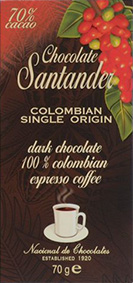
\includegraphics[scale=0.5]{Prop-32.jpg}
\end{center}
\begin{enumerate}
\item Quelle est la masse de cacao dans cette tablette de chocolat ?
\item Que signifie 100\% sur cet emballage ?
\end{enumerate}

\end{minipage}
\hfill\hfill
\begin{minipage}{0.49\linewidth}

\Exe


\begin{center}
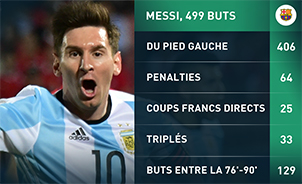
\includegraphics[scale=0.8]{Prop-35.jpg} 
\end{center}

\begin{enumerate}
\item Quel est le pourcentage de but marqués du pied gauche ?
\item Quel est le pourcentage de but marqués sur penalty ?
\item Quel est le pourcentage de but marqués entre la 76' et 90' ?
\item Pourquoi la somme des pourcentages est-elle supérieure à 100\% ? Justifie.
\end{enumerate}




\end{minipage}

\Exe



\begin{minipage}{5cm}


\includegraphics[scale=0.6]{destockage.jpg} 

\end{minipage}
\begin{minipage}{13cm}
La grande enseigne Avenueducommerce propose un déstockage sur ses produits. On peut lire "Remise immédiate de 16 \euro{} dès 101 \euro{} d'achat par tranche de 101 \euro{}".
Sa concurrente PtiBill annonce "Remise immédiate de 15\% sur tout le magasin".

Louis veut acheter une télévision qui coute 624 \euro{} chez Avenueducommerce et 610 \euro{} chez PtiBill. Dans quel magasin doit il acheter sa télévision ?

\end{minipage}






\Parcours{1}{citoyen}{Prop-25}



\begin{seance}[Proportionnalité]

\begin{description}
\item[$\square$] Résoudre des problèmes de pourcentage.
\item[$\triangleright$] Calculer des taux d'évolution.
\end{description}
\end{seance}


\begin{DefT}{Coefficient multiplicateur}\index{Coefficient multiplicateur}
Lorsque une valeur évolue selon un pourcentage de $t \%$, le coefficient multiplicateur est égal à $(1+t\%)$.
\end{DefT}

%\begin{Ex}
%\textit{La Taxe sur la Valeur Ajoutée en France est de 20,6\%. Un produit alimentaire coute 15,20 € Hors Taxe. Quel est sa valeur TTC ?}\\
%Soit P le prix du produit alimentaire.\\
%$P = 15,20 \times (1+20,6\%)= 15,20 \times (1+0,206) = 15,20 \times 1,206 \approx 18,33$.\\
%Le prix TTC est donc 18,33 €.
%\end{Ex}
%
%\begin{Ex}
%\textit{Le jour des soldes, une paire de ski à 428 € est soldée à 25\%. Quel est le prix après la solde ? }\\
%Soit P le prix de la paire de ski.\\
%$P = 428 \times (1-25\%)= 428 \times (1-0,25) = 428 \times 0,75 =321 $.\\
%Le prix soldé est donc 321 €.
%\end{Ex}


\begin{minipage}{0.47\linewidth}
\Exe


\begin{center}

\includegraphics[scale=1]{Prop-43.jpg}
\end{center}



\Exe


\begin{enumerate}
\item Augmenter de 96\% revient à multiplier par $\ldots \ldots \ldots \ldots$
\item Augmenter de 50\% revient à multiplier par $\ldots \ldots \ldots \ldots$
\item Diminuer de 25\% revient à multiplier par $\ldots \ldots \ldots \ldots$
\item Diminuer de 10\% revient à multiplier par $\ldots \ldots \ldots \ldots$
\item Augmenter de 8\% revient à multiplier par $\ldots \ldots \ldots \ldots$
\item Augmenter de 100\% revient à multiplier par $\ldots \ldots \ldots \ldots$
\item Diminuer de 35\% revient à multiplier par $\ldots \ldots \ldots \ldots$
\item Augmenter de 25\% revient à multiplier par $\ldots \ldots \ldots \ldots$
\end{enumerate}

\Exe


Fin avril 2016, en France métropolitaine, le nombre de demandeurs d'emploi tenus de rechercher un emploi et sans activité (catégorie A) s'établit à \np{3 511 100}. Ce nombre diminue de 0,6\% sur un mois. Quel était le nombre de demandeurs d'emploi le mois précédent ?

\end{minipage}
\hfill
\begin{minipage}{0.47\linewidth}

\Exe


Quel est le montant total de la facture ?

\begin{center}
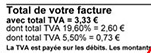
\includegraphics[scale=1]{Prop-46.jpg}
\end{center}


\Exe


\begin{enumerate}
\item Le salaire de Paul est passé de \np{1200} € à \np{1250} €. Quel est le taux d'évolution ?
\item Le salaire de Marie est passé de \np{1250} € a \np{1200} €. Quel est le taux d'évolution ?
\end{enumerate}

\Exe


Que représente en pourcentage le montant de la réduction ?

\begin{center}
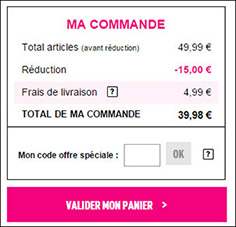
\includegraphics[scale=0.7]{Prop-45.jpg}
\end{center}

\end{minipage}

\begin{seance}[Proportionnalité]

\begin{description}
\item[$\square$] Résoudre des problèmes de pourcentage.
\item[$\triangleright$] Calculer des taux d'évolution.
\end{description}
\end{seance}

\Exe


Chaque année une association perd 10\% de ses adhérents. 

Par contre, 7 personnes prennent leur adhésion à cette association. 

Au bout de combien d'années l'association aura doublé ses adhérents ?

\Dnb


Un ouvrier doit peindre une surface totale d'environ 168 m$^2$.

 
\begin{itemize}
\item[$\bullet~~$] Un pot de 10~L de peinture permet de couvrir une surface de 40~m$^2 $ ;
\item[$\bullet~~$] Le coût d'un pot de 10~L de peinture est de 400~\euro{} ;
\item[$\bullet~~$] Un ouvrier peint une surface de 42 m$^2$ à l'heure.
\end{itemize}


 
\medskip

Compléter cette facture à l'aide des informations fournies ci-dessus.

\medskip

\begin{tabularx}{\linewidth}{|*{4}{>{\centering \arraybackslash}X|}}\hline 
\textbf{Quantité}& \textbf{Désignation} &\textbf{Prix unitaire} &\textbf{Prix total}\\ \hline 
5& pots d'antirouille &500,00~\euro&\np{2500,00}~\euro\\ \hline 
\dotfill&pots de peinture&400,00~\euro &\dotfill\\ \hline
\dotfill&\small heures (main d'{\oe}uvre)&35,00~\euro &\dotfill\\ \hline
\multicolumn{3}{|l|}{Total HT (co\^ut hors taxe)}&\dotfill\\ \hline  
\multicolumn{3}{|l|}{Montant de la TVA à 19,6\,\%}&\dotfill\\ \hline 
\multicolumn{3}{|l|}{TOTAL TTC (coût toutes taxes comprises)}&\dotfill\\ \hline
\end{tabularx}






\end{document}